% !TEX root = SystemTemplate.tex

\chapter{Overview and concept of operations}

\section{Scope}
This document will provide an overview of the develolpment of the testing software.


\section{Purpose}
This product will compile and test c++ programs against predefined test cases and give the user the option of creating additional test cases.

\section{Sprint 1}

\subsection{Major System Component \#1}
Location of existing, applicable test cases for the program needing to be tested.

\subsection{Major System Component \#2}
Run and test of a single program against located test cases

\subsection{Major System Component \#3}
Record and summary of test results

\section{Sprint 2}

\subsection{Major System Component \#4}
Process the whole class

\subsection{Major System Component \#5}
Grading system that includes critical test cases

\subsection{Major System Component \#6}
Automatic test case generation.

\section{Sprint 3}

\subsection{Major System Component \#7}
Generate lists of strings

\subsection{Major System Component \#8}
Check for infinite loops.

\subsection{Major System Component \#9}
More robust checking of answers.

\subsection{Major System Component \#10}
Menu-driven testing.

\subsection{Major System Component \#11}
Add test coverage to the report.

\subsection{Major System Component \#12}
Add performance information to the report

\section{Systems Goals}The purpose of this project is to create a program that will traverse a directory and test the necessary programs against test cases, outputting the results of the testing into a summary file.  Furthermore, the user will be able to create additional test cases according to desired requirements. The program is specifically geared toward computer science professors for the use use of grading student programs. 

\section{System Overview and Diagram}

\subsection{Sprint 1}
Upon running the application and providing it with the name of the desired target program, the application
will complete the desired system goals via its major components.
\begin{description}
\item[First      ]Existing, applicable test cases will be found for the program needing to be tested. 
\item[Second]The program will be run against each test case input, and the resulting output will be 
compared to each desired test case output.
\item[Third   ]The program will create a time-stamped record for each program tested, providing a reference of 
the output results and a numerical summary of the overall success rate.
\end{description}  
See Figure~\ref{systemdiagram} for the system overview diagram of Sprint 1.
\begin{figure}[H]
\begin{center}
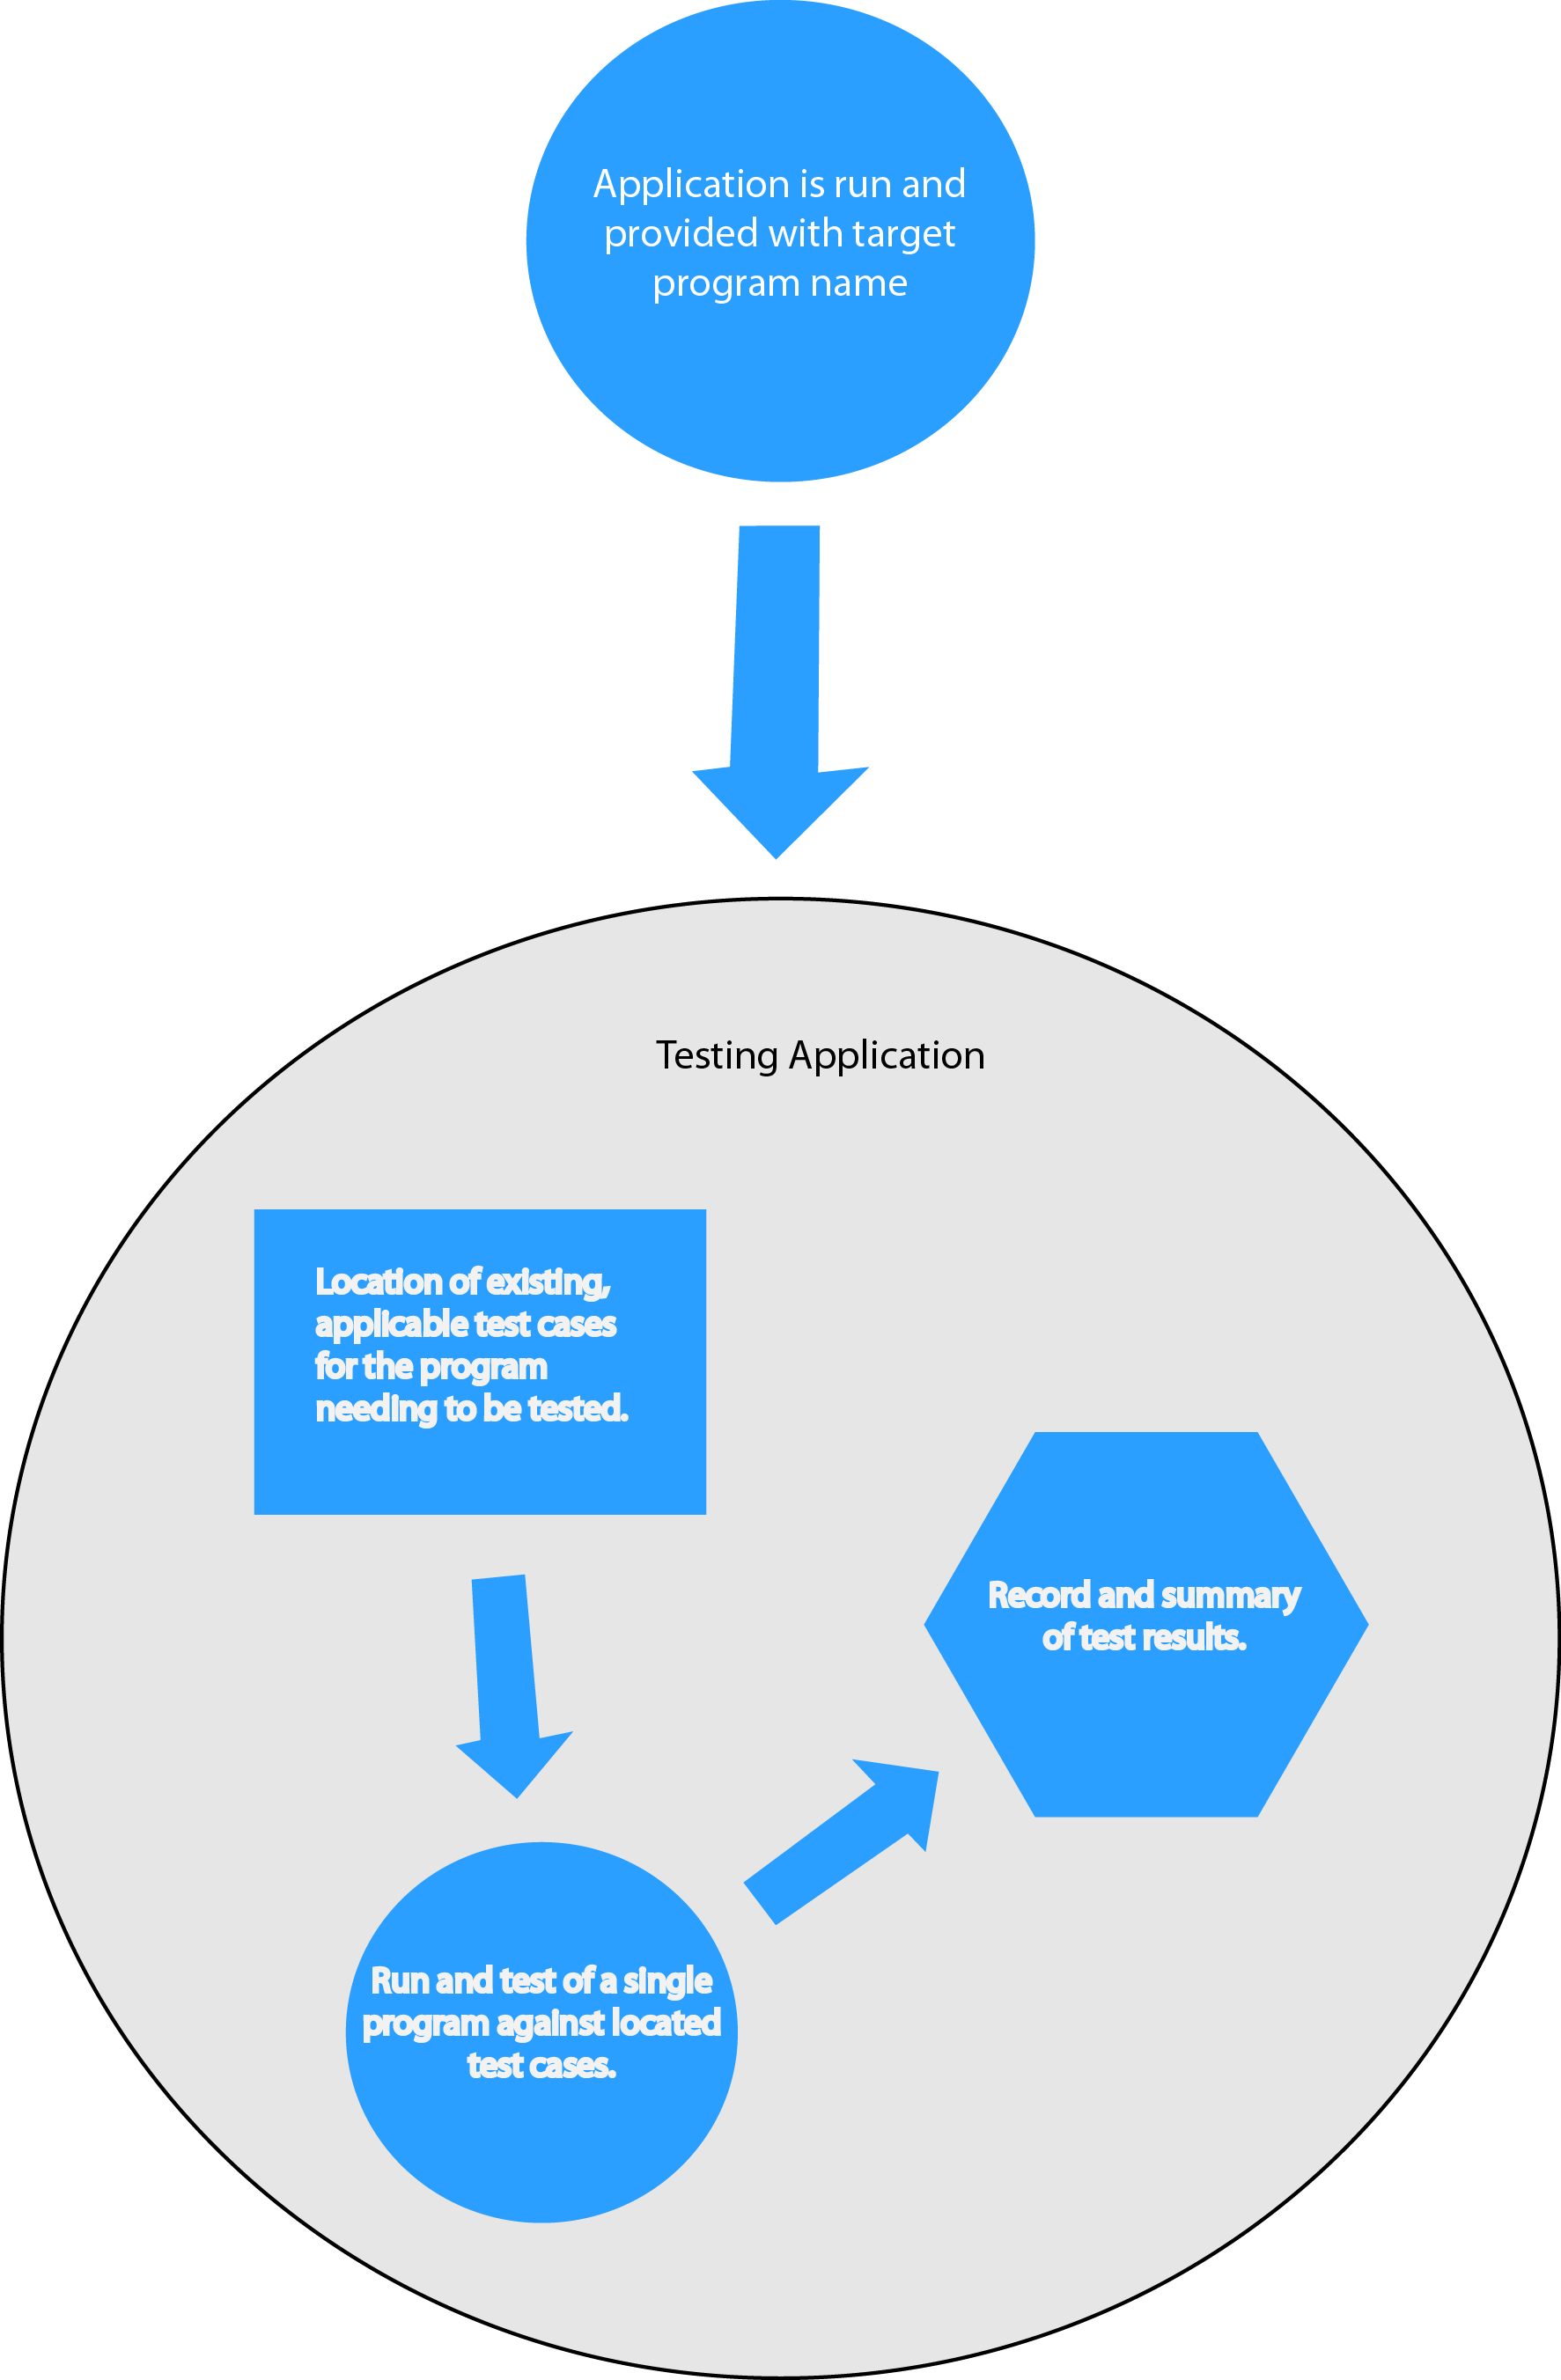
\includegraphics[width=0.5\textwidth]{./diagram}
\end{center}
\caption{The Sprint 1 Testing System Diagram \label{systemdiagram}}
\end{figure}

\subsection{Sprint 2}
Upon running the application, the user will be given a choice of either grading the programs of each student against the test cases, or generating test cases according to desired parameters.
\begin{description}
\item[First      ]The program will be able to crawl through the directory, find each student's directory, and test each student's program. See Figure~\ref{DirectoryTree} to view the directory structure.
\item[Second]The grading will now include critical test cases, which must be passed in order for a grade to be created from the success rate of the other test cases against that program.  The student's personal log and success rate will be calculated using the system created in Sprint 1. 
\item[Third   ]The user will be able to create test cases according to desired parameters, which the user will be prompted to enter.
\end{description}  
See Figure~\ref{systemdiagram2} for the system overview diagram of Sprint 2.

\begin{figure}[H]
\begin{center}
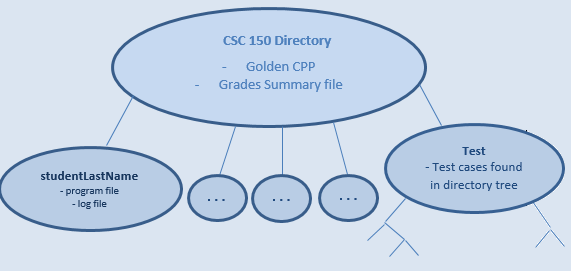
\includegraphics[width=.7\textwidth]{./DirectoryTree}
\end{center}
\caption{The Directory Structure Diagram \label{DirectoryTree}}
\end{figure}

\begin{figure}[H]
\begin{center}
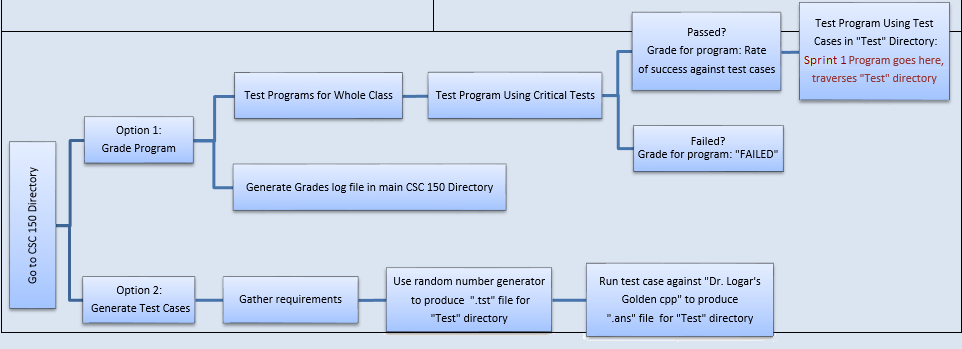
\includegraphics[width=1.1\textwidth]{./diagram2}
\end{center}
\caption{The Sprint 2 Testing System Diagram \label{systemdiagram2}}
\end{figure}

\subsection{Sprint 3}
Many features have been added in Sprint 3. 
\begin{description}
\item[First      ]The test generator of our test suite now generates string test cases.
\item[Second]Infinite loops are now prevented in the program by setting a default time limit of 60 seconds. After this time the program is terminated. This time frame can be altered by the user to be shorter or longer as needed.
\item[Third   ]Answer checking has completely evolved. Now it allows for small errors to pass with a simple notice of the errors' existence. If there are slight misspellings or incorrect spacing these will be tolerated.
\item[Fourth      ]Menu driven testing has been added as well. Instead of simply running based on single level user input the test suite is now able to handle different acceptable inputs and follow the functions logic to run the appropriate tests.
\item[Fifth   ]Test coverage as now also been implemented. This test suite now makes use of gcov to inform the user how much code is being covered by the tests run. This will enable the users to test their code more thoroughly.
\item[Six   ]Gprof is also utilized by our test suite to give the user the time spent in each function of the program being tested by the suite. This information is, as the gcov information, written to the log file of the program. 

\section{Technologies Overview}
The development team used the Agile Software Development Method, via the Scrum framework, to develop
this system.  This incremental development method was the required development method for this project.
Since the system was expected to created for a Linux platform, it was written and tested on a Linux Platform 
using Qt Creator.  The latter was picked as the Integrated Development Environment of the system, based on
the requirement that it be written in the programming language C++.
See Table~\ref{DevelopmentTable}.  
\begin{table}[tbh]
\begin{center}
\begin{tabular}{|r|l|}
  \hline
  Software Development Method & Agile Software Development Method \\
  Planning and Organization & Trello Project Management Application \\
  \hline \hline
  Platform & Linux \\
  Language & C++ \\  
  IDE & Qt Creator \\
  Version Control & GitHub and Bitbucket
  \\ \cline{2-2}
  
  \hline
\end{tabular}
\caption{The Development Methods and Technologies Table \label{DevelopmentTable}}
\end{center}
\end{table}

